\chapter{Исследовательский раздел}
\label{cha:research}

В данном разделе будут приведены замеры времени работы реализации алгоритма отрисовки сцены.
Все параметры замерялись на устройстве со следующими техническими характеристиками:
\begin{itemize}
	\item операционная система macOS Catalina 10.15.46 \cite{monterey};
	\item оперативная память 8 Гб;
	\item 1,8 ГГц 2-ядерный Intel Core i5 7 поколения \cite{intel}.
\end{itemize}

Во время замеров ноутбук был подключен к сети питания и нагружен только приложениями, использующимися при замерах.

\section{Цель эксперимента}

Цель эксперимента --- выявить зависимость времени отрисовки кадра от количества частиц вируса, находящихся на сцене. 

\section{План эксперимента}

Измерения проводятся при одной скорости движения частиц. Каждый замер производится 30 раз, а затем время усредняется.

При замерах камера не будет передвигаться и поворачиваться, не будет изменяться положение объектов на сцене.

\section{Результаты эксперимента}

Процессорное время замерялось при помощи функции std::chrono::system\_clock::now() из заголовочного файла chrono~\cite{cplusplus}. Результаты сформированы в виде графиков при помощи библиотеки matplotlib~\cite{matplotlib}. 

Результаты замеров представлены в таблице \ref{tbl:timings} и на рисунке \ref{fig:timings}.

\begin{table}[h]
	\begin{center}
		\begin{threeparttable}
			\captionsetup{justification=raggedright,singlelinecheck=off}
			\caption{\label{tbl:timings} Результаты замеров}
			\begin{tabular}{|c|c|c|}
				\hline
				Количество частиц вируса& Время отрисовки сцены (в миллисекундах) \\  \hline
				1 & 235.0 \\ \hline 
				10 & 255.0 \\ \hline 
				20 & 265.0 \\ \hline 
				40 & 295.0 \\ \hline 
				60 & 330.0 \\ \hline 
				100 & 390.0 \\ \hline 
				150 & 460.0 \\ \hline 
				200 & 550.0 \\ \hline 
				250 & 620.0 \\ \hline 
				300 & 680.0 \\ \hline 
				400 & 830.0 \\ \hline 
				500 & 1000.0 \\ \hline 
				600 & 1130.0 \\ \hline 
			\end{tabular}
		\end{threeparttable}
	\end{center}
\end{table}

На рисунке \ref{fig:timings} на оси X указано количество частиц. Время на оси Y указано в миллисекундах.

\begin{figure}[ph!]
	\center{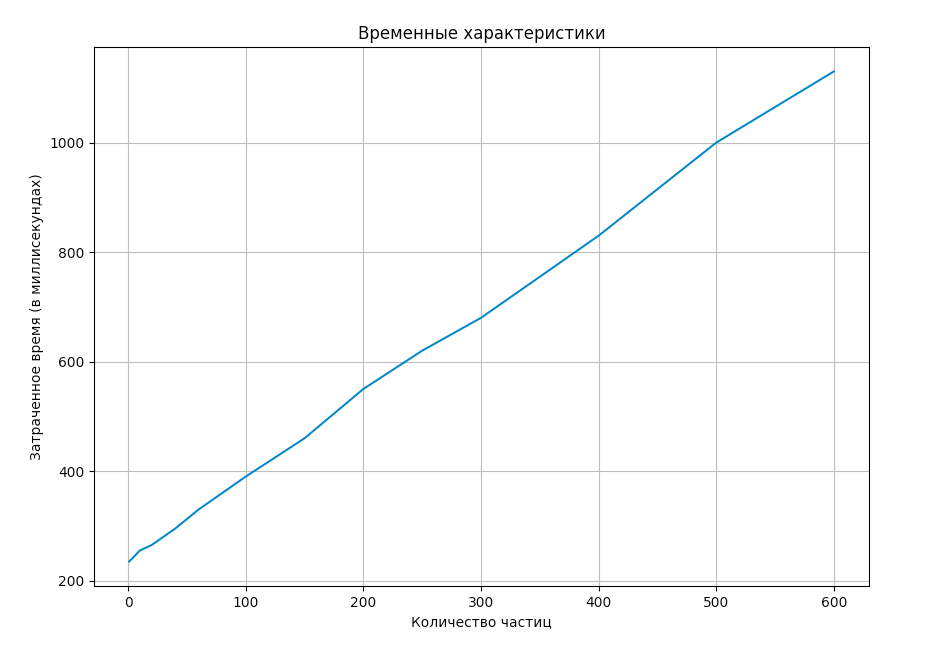
\includegraphics[scale=0.5]{img/timings.png}}
	\caption{Результаты замеров времени отрисовки кадра}
	\label{fig:timings}
\end{figure}

\clearpage

\section*{Вывод}

В результате эксперимента можно сделать вывод, что увеличение количества частиц вируса значительно влияет на скорость отрисовки изображения. Время, затрачиваемое на отрисовку сцены, линейно зависит от количества частиц.


